


\begin{figure}
    \centering
    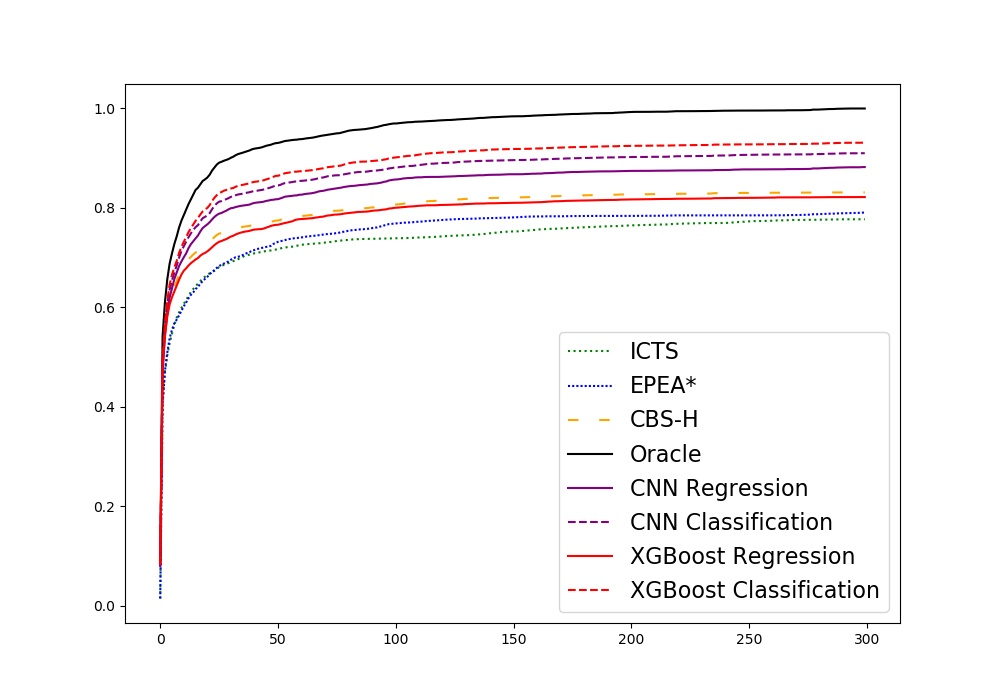
\includegraphics[width=\columnwidth]{all-cactus.jpg}
    \caption{Coverage as a function of running time over all maps}
    \label{fig:all-cactus}
\end{figure}

\Roni{Table of coverage per map}

\begin{center}
\begin{table}[t]
\resizebox{\columnwidth}{!}{
 \begin{tabular}{||l c c c c c c||} 
 \hline
 Model & City & Game & Empty & Maze & Random & Room \\ [0.25ex] 
 \hline
%  \hline
 Random & 16.07\% & 17.38\% & 17.74\% & 17.59\% & 17.32\% & 20.96\% \\ 
 \hline
 \astar & 0.05\% & 0.05\% & 0.83\% & 0.00\% & 0.87\% & 0.87\% \\ 
 \hline
 EPE\astar & 9.17\% & 5.43\% & 17.36\% & 0.00\% & 22.37\% & 5.68\% \\ 
 \hline
 ICTS & 1.24\% & 8.05\% & 18.63\% & 5.21\% & 15.26\% & 12.88\% \\ 
 \hline
 CBS & 0.10\% & 0.72\% & 0.13\% & 0.98\% & 0.25\% & 1.75\% \\ 
 \hline
 MA-CBS & 21.69\% & 22.26\% & 43.52\% & 23.78\% & 23.61\% & 18.12\% \\ 
 \hline
 CBS-H & 67.75\% & 63.48\% & 19.53\% & \textbf{70.03}\% & 37.63\% & 60.70\% \\ 
 \hline
 CNN Rg. & 56.44\% & 62.08\% & 43.39\% & 63.84\% & 37.81\% & 45.85\% \\ 
 \hline
 CNN Cl. & 67.74\% & 63.48\% & 28.97\% & \textbf{70.03}\% & 47.47\% & 60.69\% \\ 
 \hline
XGBoost Rg. & 12.26\% & 18.09\% & 10.08\% & 8.79\% & 9.90\% & 9.60\% \\ 
 \hline
 XGBoost Cl. & \textbf{71.95}\% & \textbf{87.23}\% & \textbf{78.18}\% & 67.41\% & 51.21\% & \textbf{66.59}\% \\ 
 \hline
\end{tabular}
}
\label{table:acc-per-map}
\caption{Accuracy results, split by grid type.}
\end{table}
\end{center}

\begin{center}
\begin{table}[t]
\resizebox{\columnwidth}{!}{
 \begin{tabular}{||l c c c c c c||} 
 \hline
 Model & City & Game & Empty & Maze & Random & Room \\ [0.25ex] 
 \hline
%  \hline
 Random & 65.38\% & 68.51\% & 74.92\% & 84.04\% & 70.47\% & 82.97\% \\ 
 \hline
  \astar & 65.69\% & 68.64\% & 85.00\% & 77.52\% & 74.21\% & 78.17\% \\ 
 \hline
 EPE\astar & 66.87\% & 71.99\% & 94.95\% & 79.15\% & 88.04\% & 81.00\% \\ 
 \hline
 ICTS & 70.89\% & 72.08\% & 83.60\% & 81.76\% & 85.86\% & 82.75\% \\ 
 \hline
 CBS & 55.33\% & 55.57\% & 59.60\% & 86.97\% & 55.02\% & 84.93\% \\ 
 \hline
 MA-CBS & 45.85\% & 49.23\% & 57.75\% & 77.52\% & 50.90\% & 68.34\% \\ 
 \hline
  CBS-H & \textbf{91.34}\% & 90.68\% & 67.45\% & \textbf{99.02}\% & 71.28\% & \textbf{96.29}\% \\ 
 \hline
 CNN Rg. & 77.33\% & 91.99\% & \textbf{96.10}\% & 94.14\% & 87.53\% & 87.55\% \\ 
 \hline
 CNN Cl. & \textbf{91.34}\% & 90.67\% & 88.13\% & \textbf{99.02}\% & \textbf{90.84}\% & 96.28\% \\ 
 \hline
XGBoost Rg. & 86.40\% & 89.68\% & 68.86\% & 96.74\% & 69.28\% & 91.05\% \\ 
 \hline
 XGBoost Cl. & 87.07\% & \textbf{92.22}\% & 90.24\% & 97.07\% & 90.09\% & \textbf{96.29}\% \\ 
 \hline 
\end{tabular}
}
\label{table:coverage-map}
\caption{Coverage results of models per map type  }
\end{table}
\end{center}


% Cactus per map
\Roni{Cactus per map, showing EPEA*, ICTS, CBS-H, and our Algorithm Selection algorithms, and Oracle}

% Feature importance
\Roni{Feature importance only for the best classification algorithm. Show only for one algorithm. One time for all. One time per map}
